\documentclass[a4paper,twoside,11pt]{article}
\usepackage[utf8]{inputenc}
\usepackage[portuguese]{babel}
\usepackage{graphicx}
\usepackage{url}
\usepackage{titlesec}


% Redefinição das margens das páginas
\setlength{\textheight}{24.00cm}
\setlength{\textwidth}{15.50cm}
\setlength{\topmargin}{0.35cm}
\setlength{\headheight}{0cm}
\setlength{\headsep}{0cm}
\setlength{\oddsidemargin}{0.25cm}
\setlength{\evensidemargin}{0.25cm}
\setlength{\parindent}{0pt}

\begin{document}

\vspace{-15mm}
\begin{figure}[h]
\begin{center}
\resizebox{80mm}{!}{
\includegraphics{logoISEL.png}}
\end{center}
\end{figure}
\vspace{-8mm}

% Title Section
\begin{center}
    \LARGE \textbf{LiftDrop} \\ % Bold title
    \LARGE Mobile App for Deliveries \\ % Subtitle in normal weight
    \vspace{8mm}
    \large Gonçalo Morais, n.º 49502, e-mail: a49502@alunos.isel.pt, tel.: 927468061 \\
    \vspace{1mm}
    \large João Ramos, n.º 49424, e-mail: a49424@alunos.isel.pt, tel.: 919222551 \\
    \vspace{5mm}
    \large \textbf{Orientador:} Miguel Gamboa, e-mail: miguel.gamboa@isel.pt \\
    \vspace{3mm}
    \large \textbf{Co-Orientador:} Diogo Silva, e-mail: diogo.silva@lyzer.tech \\
    \vspace{5mm}
    \textbf{Março de 2025}
\end{center}

\vspace{10mm}

{\sffamily
\section*{Introduction}

\vspace{5mm}

\subsection*{Contextualization}

\vspace{3mm}

The rise of the \textbf{gig economy} has transformed various industries, particularly in the food delivery sector. This economic model is characterized by short-term, flexible work arrangements where individuals take on temporary jobs, often facilitated through digital platforms. Companies such as \textbf{Uber Eats, Glovo, and Bolt Food} have leveraged this framework to revolutionize urban logistics, enabling customers to order food on demand while providing couriers with independent work opportunities.

\vspace{5mm}

By prioritizing \textbf{customer convenience}, these platforms have successfully streamlined food delivery processes through real-time technology, ensuring efficiency and reliability at scale. However, as demand for delivery services continues to grow, the gig economy also presents operational challenges, particularly affecting the couriers who sustain this system.

\section*{Project Goals}

To address these challenges, this project aims to develop a delivery-focused mobile application that enhances the working experience of couriers by:

\begin{itemize}
    \item \textbf{Enhancing decision-making} by providing couriers with \textbf{real-time demand insights} through heat maps that highlight high-order density areas.
    \item \textbf{Increasing courier safety} by implementing a \textbf{safety rating system} for neighborhoods and delivery areas.
    \item \textbf{Enabling earnings tracking} (Optional) to help couriers monitor income and performance trends.
\end{itemize}

}

\section*{Research}

Developing a delivery-focused mobile application presents challenges, particularly in real-time data handling and order assignment. Since multiple couriers interact with the platform simultaneously, the system must manage updates effectively while ensuring a smooth user experience. After some research and consideration, we identified two primary approaches to handling real-time updates and concurrency:

\begin{itemize}
    \item \textbf{Polling-based Request-Response Model}, where the client periodically requests updates from the server. While simple to implement, this approach leads to unnecessary network requests, increased server load, and delayed updates.
    \item \textbf{Event-Driven Server-Sent Events (SSE)}, where the server pushes updates to clients as they occur. This enables real-time communication without the inefficiencies of constant polling.
\end{itemize}

We chose SSE for real-time updates due to its reliability and maintainability. To implement Server-Sent Events (SSE), we'll use OkHttp to manage the connection, as Android lacks native SSE support. This ensures real-time updates without the inefficiencies of polling.

\vspace{2mm}

For order assignment, the platform will consider factors like \textbf{Proximity-based allocation}, \textbf{Fair distribution}, and \textbf{Traffic-aware routing}. An external geospatial API will handle location-based calculations (distance, routing, and traffic), simplifying the implementation by reducing the need for complex in-house geospatial logic.

\vspace{2mm}

To address safety concerns, the platform will integrate features such as neighborhood safety ratings, which provide security indicators based on user feedback. Couriers will receive alerts when accepting deliveries in high-risk areas. Additionally, nighttime safety measures will offer visibility into risk-prone areas for deliveries made late at night.


\section*{Architecture and Tools (TO DO)}

The system architecture will consist of the following components:

\begin{itemize}
\item \textbf{Application for Android}: Implements the user interface and core functionality for couriers.
\item \textbf{Web API}: Provides backend logic and data management for real-time interactions.
\item \textbf{Database}: Stores connections between entities along with additional order and user-related data.
\end{itemize}

This architecture provides a robust and scalable foundation for the system, ensuring seamless interaction between the Android application, web API, and database.

\subsection*{Challenges Ahead (TO DO)}

\newpage

\section*{Project Plan}

\begin{figure}[h]
    \centering
    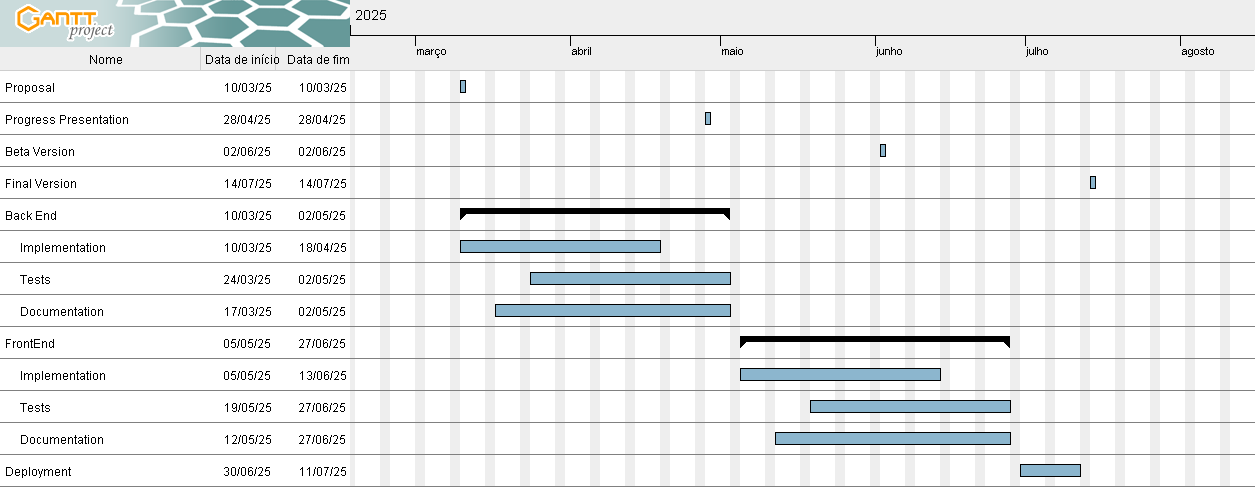
\includegraphics[width=\textwidth]{ProjectPlan.png}
    \caption{Project Plan}
    \label{fig:project-plan}
\end{figure}

\bibliographystyle{alpha}
\bibliography{sample}


\end{document}